\documentclass[twoside]{book}

% Packages required by doxygen
\usepackage{fixltx2e}
\usepackage{calc}
\usepackage{doxygen}
\usepackage[export]{adjustbox} % also loads graphicx
\usepackage{graphicx}
\usepackage[utf8]{inputenc}
\usepackage{makeidx}
\usepackage{multicol}
\usepackage{multirow}
\PassOptionsToPackage{warn}{textcomp}
\usepackage{textcomp}
\usepackage[nointegrals]{wasysym}
\usepackage[table]{xcolor}

% Font selection
\usepackage[T1]{fontenc}
\usepackage[scaled=.90]{helvet}
\usepackage{courier}
\usepackage{amssymb}
\usepackage{sectsty}
\renewcommand{\familydefault}{\sfdefault}
\allsectionsfont{%
  \fontseries{bc}\selectfont%
  \color{darkgray}%
}
\renewcommand{\DoxyLabelFont}{%
  \fontseries{bc}\selectfont%
  \color{darkgray}%
}
\newcommand{\+}{\discretionary{\mbox{\scriptsize$\hookleftarrow$}}{}{}}

% Page & text layout
\usepackage{geometry}
\geometry{%
  a4paper,%
  top=2.5cm,%
  bottom=2.5cm,%
  left=2.5cm,%
  right=2.5cm%
}
\tolerance=750
\hfuzz=15pt
\hbadness=750
\setlength{\emergencystretch}{15pt}
\setlength{\parindent}{0cm}
\setlength{\parskip}{3ex plus 2ex minus 2ex}
\makeatletter
\renewcommand{\paragraph}{%
  \@startsection{paragraph}{4}{0ex}{-1.0ex}{1.0ex}{%
    \normalfont\normalsize\bfseries\SS@parafont%
  }%
}
\renewcommand{\subparagraph}{%
  \@startsection{subparagraph}{5}{0ex}{-1.0ex}{1.0ex}{%
    \normalfont\normalsize\bfseries\SS@subparafont%
  }%
}
\makeatother

% Headers & footers
\usepackage{fancyhdr}
\pagestyle{fancyplain}
\fancyhead[LE]{\fancyplain{}{\bfseries\thepage}}
\fancyhead[CE]{\fancyplain{}{}}
\fancyhead[RE]{\fancyplain{}{\bfseries\leftmark}}
\fancyhead[LO]{\fancyplain{}{\bfseries\rightmark}}
\fancyhead[CO]{\fancyplain{}{}}
\fancyhead[RO]{\fancyplain{}{\bfseries\thepage}}
\fancyfoot[LE]{\fancyplain{}{}}
\fancyfoot[CE]{\fancyplain{}{}}
\fancyfoot[RE]{\fancyplain{}{\bfseries\scriptsize Generated by Doxygen }}
\fancyfoot[LO]{\fancyplain{}{\bfseries\scriptsize Generated by Doxygen }}
\fancyfoot[CO]{\fancyplain{}{}}
\fancyfoot[RO]{\fancyplain{}{}}
\renewcommand{\footrulewidth}{0.4pt}
\renewcommand{\chaptermark}[1]{%
  \markboth{#1}{}%
}
\renewcommand{\sectionmark}[1]{%
  \markright{\thesection\ #1}%
}

% Indices & bibliography
\usepackage{natbib}
\usepackage[titles]{tocloft}
\setcounter{tocdepth}{3}
\setcounter{secnumdepth}{5}
\makeindex

% Hyperlinks (required, but should be loaded last)
\usepackage{ifpdf}
\ifpdf
  \usepackage[pdftex,pagebackref=true]{hyperref}
\else
  \usepackage[ps2pdf,pagebackref=true]{hyperref}
\fi
\hypersetup{%
  colorlinks=true,%
  linkcolor=blue,%
  citecolor=blue,%
  unicode%
}

% Custom commands
\newcommand{\clearemptydoublepage}{%
  \newpage{\pagestyle{empty}\cleardoublepage}%
}

\usepackage{caption}
\captionsetup{labelsep=space,justification=centering,font={bf},singlelinecheck=off,skip=4pt,position=top}

%===== C O N T E N T S =====

\begin{document}

% Titlepage & ToC
\hypersetup{pageanchor=false,
             bookmarksnumbered=true,
             pdfencoding=unicode
            }
\pagenumbering{alph}
\begin{titlepage}
\vspace*{7cm}
\begin{center}%
{\Large Bank\+App }\\
\vspace*{1cm}
{\large Generated by Doxygen 1.8.13}\\
\end{center}
\end{titlepage}
\clearemptydoublepage
\pagenumbering{roman}
\tableofcontents
\clearemptydoublepage
\pagenumbering{arabic}
\hypersetup{pageanchor=true}

%--- Begin generated contents ---
\chapter{Bank application as a project for S\+O\+F\+T\+W\+A\+RE P\+R\+O\+C\+E\+SS A\+ND Q\+U\+A\+L\+I\+TY}
\label{index}\hypertarget{index}{}This is the main Login Class\begin{DoxyAuthor}{Author}
B\+I\+C\+H\+RI
\end{DoxyAuthor}
\begin{DoxyDate}{Date}
05-\/17-\/2017
\end{DoxyDate}
\begin{DoxyWarning}{Warning}
This code is Just a school project, not for professional use
\end{DoxyWarning}
\begin{DoxyCopyright}{Copyright}
Free license
\end{DoxyCopyright}
\hypertarget{index_intro_sec}{}\section{Introduction}\label{index_intro_sec}
this an apllication to help users and managers to do their daily tasks easily\hypertarget{index_compile_sec}{}\section{Compilation}\label{index_compile_sec}
know how to compile the code using maven 
\chapter{Hierarchical Index}
\section{Class Hierarchy}
This inheritance list is sorted roughly, but not completely, alphabetically\+:\begin{DoxyCompactList}
\item \contentsline{section}{bankapp.\+server.\+Account}{\pageref{classbankapp_1_1server_1_1_account}}{}
\begin{DoxyCompactList}
\item \contentsline{section}{bankapp.\+server.\+Admin}{\pageref{classbankapp_1_1server_1_1_admin}}{}
\item \contentsline{section}{bankapp.\+server.\+User}{\pageref{classbankapp_1_1server_1_1_user}}{}
\end{DoxyCompactList}
\item \contentsline{section}{bankapp.\+server.\+bank\+Account}{\pageref{classbankapp_1_1server_1_1bank_account}}{}
\item \contentsline{section}{bankapp.\+server.\+bank\+Account\+Test}{\pageref{classbankapp_1_1server_1_1bank_account_test}}{}
\item \contentsline{section}{bankapp.\+client.\+bank\+Client}{\pageref{classbankapp_1_1client_1_1bank_client}}{}
\item \contentsline{section}{bankapp.\+client.\+bank\+Controller}{\pageref{classbankapp_1_1client_1_1bank_controller}}{}
\item \contentsline{section}{bankapp.\+server.\+bank\+Server}{\pageref{classbankapp_1_1server_1_1bank_server}}{}
\item \contentsline{section}{bankapp.\+server.\+B\+D\+Test}{\pageref{classbankapp_1_1server_1_1_b_d_test}}{}
\item \contentsline{section}{bankapp.\+server.\+Ibank\+D\+AO}{\pageref{interfacebankapp_1_1server_1_1_ibank_d_a_o}}{}
\begin{DoxyCompactList}
\item \contentsline{section}{bankapp.\+server.\+bank\+D\+AO}{\pageref{classbankapp_1_1server_1_1bank_d_a_o}}{}
\end{DoxyCompactList}
\item \contentsline{section}{bankapp.\+server.\+Performance}{\pageref{classbankapp_1_1server_1_1_performance}}{}
\item \contentsline{section}{bankapp.\+server.\+Report}{\pageref{classbankapp_1_1server_1_1_report}}{}
\item \contentsline{section}{bankapp.\+server.\+Report\+Test}{\pageref{classbankapp_1_1server_1_1_report_test}}{}
\item \contentsline{section}{bankapp.\+client.\+R\+M\+I\+Service\+Locator}{\pageref{classbankapp_1_1client_1_1_r_m_i_service_locator}}{}
\item \contentsline{section}{bankapp.\+server.\+Server\+Test}{\pageref{classbankapp_1_1server_1_1_server_test}}{}
\item \contentsline{section}{bankapp.\+server.\+User\+Test}{\pageref{classbankapp_1_1server_1_1_user_test}}{}
\item Remote\begin{DoxyCompactList}
\item \contentsline{section}{bankapp.\+server.\+I\+B\+Manager}{\pageref{interfacebankapp_1_1server_1_1_i_b_manager}}{}
\begin{DoxyCompactList}
\item \contentsline{section}{bankapp.\+server.\+B\+Manager}{\pageref{classbankapp_1_1server_1_1_b_manager}}{}
\end{DoxyCompactList}
\end{DoxyCompactList}
\item Unicast\+Remote\+Object\begin{DoxyCompactList}
\item \contentsline{section}{bankapp.\+server.\+B\+Manager}{\pageref{classbankapp_1_1server_1_1_b_manager}}{}
\end{DoxyCompactList}
\end{DoxyCompactList}

\chapter{Class Index}
\section{Class List}
Here are the classes, structs, unions and interfaces with brief descriptions\+:\begin{DoxyCompactList}
\item\contentsline{section}{\hyperlink{classbankapp_1_1server_1_1_account}{bankapp.\+server.\+Account} }{\pageref{classbankapp_1_1server_1_1_account}}{}
\item\contentsline{section}{\hyperlink{classbankapp_1_1server_1_1_admin}{bankapp.\+server.\+Admin} }{\pageref{classbankapp_1_1server_1_1_admin}}{}
\item\contentsline{section}{\hyperlink{classbankapp_1_1server_1_1bank_account}{bankapp.\+server.\+bank\+Account} }{\pageref{classbankapp_1_1server_1_1bank_account}}{}
\item\contentsline{section}{\hyperlink{classbankapp_1_1server_1_1bank_account_test}{bankapp.\+server.\+bank\+Account\+Test} }{\pageref{classbankapp_1_1server_1_1bank_account_test}}{}
\item\contentsline{section}{\hyperlink{classbankapp_1_1client_1_1bank_client}{bankapp.\+client.\+bank\+Client} }{\pageref{classbankapp_1_1client_1_1bank_client}}{}
\item\contentsline{section}{\hyperlink{classbankapp_1_1client_1_1bank_controller}{bankapp.\+client.\+bank\+Controller} }{\pageref{classbankapp_1_1client_1_1bank_controller}}{}
\item\contentsline{section}{\hyperlink{classbankapp_1_1server_1_1bank_d_a_o}{bankapp.\+server.\+bank\+D\+AO} }{\pageref{classbankapp_1_1server_1_1bank_d_a_o}}{}
\item\contentsline{section}{\hyperlink{classbankapp_1_1server_1_1bank_server}{bankapp.\+server.\+bank\+Server} }{\pageref{classbankapp_1_1server_1_1bank_server}}{}
\item\contentsline{section}{\hyperlink{classbankapp_1_1server_1_1_b_d_test}{bankapp.\+server.\+B\+D\+Test} }{\pageref{classbankapp_1_1server_1_1_b_d_test}}{}
\item\contentsline{section}{\hyperlink{classbankapp_1_1server_1_1_b_manager}{bankapp.\+server.\+B\+Manager} }{\pageref{classbankapp_1_1server_1_1_b_manager}}{}
\item\contentsline{section}{\hyperlink{interfacebankapp_1_1server_1_1_ibank_d_a_o}{bankapp.\+server.\+Ibank\+D\+AO} }{\pageref{interfacebankapp_1_1server_1_1_ibank_d_a_o}}{}
\item\contentsline{section}{\hyperlink{interfacebankapp_1_1server_1_1_i_b_manager}{bankapp.\+server.\+I\+B\+Manager} }{\pageref{interfacebankapp_1_1server_1_1_i_b_manager}}{}
\item\contentsline{section}{\hyperlink{classbankapp_1_1server_1_1_performance}{bankapp.\+server.\+Performance} }{\pageref{classbankapp_1_1server_1_1_performance}}{}
\item\contentsline{section}{\hyperlink{classbankapp_1_1server_1_1_report}{bankapp.\+server.\+Report} }{\pageref{classbankapp_1_1server_1_1_report}}{}
\item\contentsline{section}{\hyperlink{classbankapp_1_1server_1_1_report_test}{bankapp.\+server.\+Report\+Test} }{\pageref{classbankapp_1_1server_1_1_report_test}}{}
\item\contentsline{section}{\hyperlink{classbankapp_1_1client_1_1_r_m_i_service_locator}{bankapp.\+client.\+R\+M\+I\+Service\+Locator} }{\pageref{classbankapp_1_1client_1_1_r_m_i_service_locator}}{}
\item\contentsline{section}{\hyperlink{classbankapp_1_1server_1_1_server_test}{bankapp.\+server.\+Server\+Test} }{\pageref{classbankapp_1_1server_1_1_server_test}}{}
\item\contentsline{section}{\hyperlink{classbankapp_1_1server_1_1_user}{bankapp.\+server.\+User} }{\pageref{classbankapp_1_1server_1_1_user}}{}
\item\contentsline{section}{\hyperlink{classbankapp_1_1server_1_1_user_test}{bankapp.\+server.\+User\+Test} }{\pageref{classbankapp_1_1server_1_1_user_test}}{}
\end{DoxyCompactList}

\chapter{Class Documentation}
\hypertarget{classes_1_1deusto_1_1spq_1_1AppTest}{}\section{es.\+deusto.\+spq.\+App\+Test Class Reference}
\label{classes_1_1deusto_1_1spq_1_1AppTest}\index{es.\+deusto.\+spq.\+App\+Test@{es.\+deusto.\+spq.\+App\+Test}}


class Unit test for simple App.  


Inheritance diagram for es.\+deusto.\+spq.\+App\+Test\+:\begin{figure}[H]
\begin{center}
\leavevmode
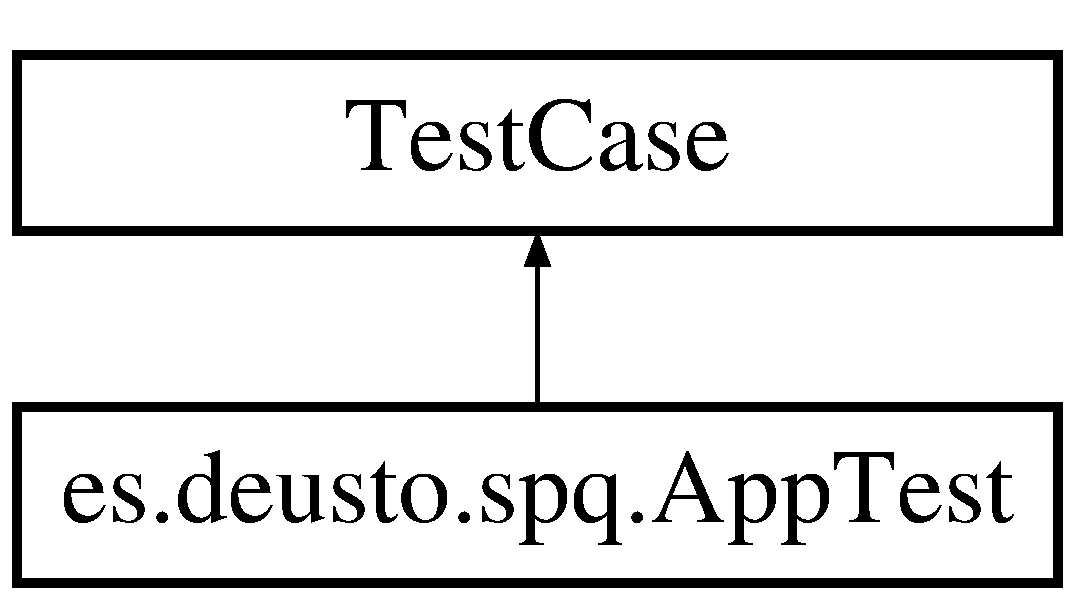
\includegraphics[height=2.000000cm]{classes_1_1deusto_1_1spq_1_1AppTest}
\end{center}
\end{figure}
\subsection*{Public Member Functions}
\begin{DoxyCompactItemize}
\item 
\hyperlink{classes_1_1deusto_1_1spq_1_1AppTest_a972284322afe0fcb22d82f0209af089a}{App\+Test} (String test\+Name)
\begin{DoxyCompactList}\small\item\em Create the test case. \end{DoxyCompactList}\item 
\mbox{\Hypertarget{classes_1_1deusto_1_1spq_1_1AppTest_afe47d45327289bf35acf77252c8e5273}\label{classes_1_1deusto_1_1spq_1_1AppTest_afe47d45327289bf35acf77252c8e5273}} 
void \hyperlink{classes_1_1deusto_1_1spq_1_1AppTest_afe47d45327289bf35acf77252c8e5273}{test\+App} ()
\begin{DoxyCompactList}\small\item\em Rigourous Test. \end{DoxyCompactList}\end{DoxyCompactItemize}
\subsection*{Static Public Member Functions}
\begin{DoxyCompactItemize}
\item 
static Test \hyperlink{classes_1_1deusto_1_1spq_1_1AppTest_ac59db16cf8210db66a8f053d62f455f8}{suite} ()
\end{DoxyCompactItemize}


\subsection{Detailed Description}
class Unit test for simple App. 

\begin{DoxyAuthor}{Author}
B\+I\+C\+H\+RI 
\end{DoxyAuthor}
\begin{DoxyDate}{Date}
05-\/17-\/2017 
\end{DoxyDate}


\subsection{Constructor \& Destructor Documentation}
\mbox{\Hypertarget{classes_1_1deusto_1_1spq_1_1AppTest_a972284322afe0fcb22d82f0209af089a}\label{classes_1_1deusto_1_1spq_1_1AppTest_a972284322afe0fcb22d82f0209af089a}} 
\index{es\+::deusto\+::spq\+::\+App\+Test@{es\+::deusto\+::spq\+::\+App\+Test}!App\+Test@{App\+Test}}
\index{App\+Test@{App\+Test}!es\+::deusto\+::spq\+::\+App\+Test@{es\+::deusto\+::spq\+::\+App\+Test}}
\subsubsection{\texorpdfstring{App\+Test()}{AppTest()}}
{\footnotesize\ttfamily es.\+deusto.\+spq.\+App\+Test.\+App\+Test (\begin{DoxyParamCaption}\item[{String}]{test\+Name }\end{DoxyParamCaption})}



Create the test case. 


\begin{DoxyParams}{Parameters}
{\em test\+Name} & name of the test case \\
\hline
\end{DoxyParams}


\subsection{Member Function Documentation}
\mbox{\Hypertarget{classes_1_1deusto_1_1spq_1_1AppTest_ac59db16cf8210db66a8f053d62f455f8}\label{classes_1_1deusto_1_1spq_1_1AppTest_ac59db16cf8210db66a8f053d62f455f8}} 
\index{es\+::deusto\+::spq\+::\+App\+Test@{es\+::deusto\+::spq\+::\+App\+Test}!suite@{suite}}
\index{suite@{suite}!es\+::deusto\+::spq\+::\+App\+Test@{es\+::deusto\+::spq\+::\+App\+Test}}
\subsubsection{\texorpdfstring{suite()}{suite()}}
{\footnotesize\ttfamily static Test es.\+deusto.\+spq.\+App\+Test.\+suite (\begin{DoxyParamCaption}{ }\end{DoxyParamCaption})\hspace{0.3cm}{\ttfamily [static]}}

\begin{DoxyReturn}{Returns}
the suite of tests being tested 
\end{DoxyReturn}


The documentation for this class was generated from the following file\+:\begin{DoxyCompactItemize}
\item 
Bank\+App/src/test/java/es/deusto/spq/App\+Test.\+java\end{DoxyCompactItemize}

\hypertarget{classbankapp_1_1client_1_1bankClient}{}\section{bankapp.\+client.\+bank\+Client Class Reference}
\label{classbankapp_1_1client_1_1bankClient}\index{bankapp.\+client.\+bank\+Client@{bankapp.\+client.\+bank\+Client}}
\subsection*{Static Public Member Functions}
\begin{DoxyCompactItemize}
\item 
static void \hyperlink{classbankapp_1_1client_1_1bankClient_ad22392d35ad10f91cc417f169b69ff7b}{main} (String\mbox{[}$\,$\mbox{]} args)
\begin{DoxyCompactList}\small\item\em main fuction that will print outputs and get inputs to identify the user \end{DoxyCompactList}\end{DoxyCompactItemize}


\subsection{Member Function Documentation}
\mbox{\Hypertarget{classbankapp_1_1client_1_1bankClient_ad22392d35ad10f91cc417f169b69ff7b}\label{classbankapp_1_1client_1_1bankClient_ad22392d35ad10f91cc417f169b69ff7b}} 
\index{bankapp\+::client\+::bank\+Client@{bankapp\+::client\+::bank\+Client}!main@{main}}
\index{main@{main}!bankapp\+::client\+::bank\+Client@{bankapp\+::client\+::bank\+Client}}
\subsubsection{\texorpdfstring{main()}{main()}}
{\footnotesize\ttfamily static void bankapp.\+client.\+bank\+Client.\+main (\begin{DoxyParamCaption}\item[{String \mbox{[}$\,$\mbox{]}}]{args }\end{DoxyParamCaption})\hspace{0.3cm}{\ttfamily [static]}}



main fuction that will print outputs and get inputs to identify the user 


\begin{DoxyParams}{Parameters}
{\em args} & \\
\hline
\end{DoxyParams}


The documentation for this class was generated from the following file\+:\begin{DoxyCompactItemize}
\item 
Bank\+App/src/main/java/bankapp/client/bank\+Client.\+java\end{DoxyCompactItemize}

\hypertarget{classbankapp_1_1client_1_1bankController}{}\section{bankapp.\+client.\+bank\+Controller Class Reference}
\label{classbankapp_1_1client_1_1bankController}\index{bankapp.\+client.\+bank\+Controller@{bankapp.\+client.\+bank\+Controller}}


This is the bank controller and hundler Class.  


\subsection*{Public Member Functions}
\begin{DoxyCompactItemize}
\item 
\hyperlink{classbankapp_1_1client_1_1bankController_a632bf32141520837c5c06a2657a7c230}{bank\+Controller} (String ip, String port, String service\+Name)
\begin{DoxyCompactList}\small\item\em Constructor set the service for the R\+MI. \end{DoxyCompactList}\item 
boolean \hyperlink{classbankapp_1_1client_1_1bankController_aed80209fad3f3fee830107d259afb445}{login} (String user, String pass)
\begin{DoxyCompactList}\small\item\em Login Function Allow or Deny access to the application. \end{DoxyCompactList}\end{DoxyCompactItemize}


\subsection{Detailed Description}
This is the bank controller and hundler Class. 

\begin{DoxyAuthor}{Author}
B\+I\+C\+H\+RI 
\end{DoxyAuthor}
\begin{DoxyDate}{Date}
05-\/17-\/2017 
\end{DoxyDate}


\subsection{Constructor \& Destructor Documentation}
\mbox{\Hypertarget{classbankapp_1_1client_1_1bankController_a632bf32141520837c5c06a2657a7c230}\label{classbankapp_1_1client_1_1bankController_a632bf32141520837c5c06a2657a7c230}} 
\index{bankapp\+::client\+::bank\+Controller@{bankapp\+::client\+::bank\+Controller}!bank\+Controller@{bank\+Controller}}
\index{bank\+Controller@{bank\+Controller}!bankapp\+::client\+::bank\+Controller@{bankapp\+::client\+::bank\+Controller}}
\subsubsection{\texorpdfstring{bank\+Controller()}{bankController()}}
{\footnotesize\ttfamily bankapp.\+client.\+bank\+Controller.\+bank\+Controller (\begin{DoxyParamCaption}\item[{String}]{ip,  }\item[{String}]{port,  }\item[{String}]{service\+Name }\end{DoxyParamCaption})}



Constructor set the service for the R\+MI. 


\begin{DoxyParams}{Parameters}
{\em ip} & \\
\hline
{\em port} & \\
\hline
{\em service\+Name} & \\
\hline
\end{DoxyParams}


\subsection{Member Function Documentation}
\mbox{\Hypertarget{classbankapp_1_1client_1_1bankController_aed80209fad3f3fee830107d259afb445}\label{classbankapp_1_1client_1_1bankController_aed80209fad3f3fee830107d259afb445}} 
\index{bankapp\+::client\+::bank\+Controller@{bankapp\+::client\+::bank\+Controller}!login@{login}}
\index{login@{login}!bankapp\+::client\+::bank\+Controller@{bankapp\+::client\+::bank\+Controller}}
\subsubsection{\texorpdfstring{login()}{login()}}
{\footnotesize\ttfamily boolean bankapp.\+client.\+bank\+Controller.\+login (\begin{DoxyParamCaption}\item[{String}]{user,  }\item[{String}]{pass }\end{DoxyParamCaption})}



Login Function Allow or Deny access to the application. 


\begin{DoxyParams}{Parameters}
{\em user} & \\
\hline
{\em pass} & \\
\hline
\end{DoxyParams}
\begin{DoxyReturn}{Returns}
true 
\end{DoxyReturn}


The documentation for this class was generated from the following file\+:\begin{DoxyCompactItemize}
\item 
Bank\+App/src/main/java/bankapp/client/bank\+Controller.\+java\end{DoxyCompactItemize}

\hypertarget{classbankapp_1_1server_1_1bankDAO}{}\section{bankapp.\+server.\+bank\+D\+AO Class Reference}
\label{classbankapp_1_1server_1_1bankDAO}\index{bankapp.\+server.\+bank\+D\+AO@{bankapp.\+server.\+bank\+D\+AO}}


This is the bank D\+AO Class.  


Inheritance diagram for bankapp.\+server.\+bank\+D\+AO\+:\begin{figure}[H]
\begin{center}
\leavevmode
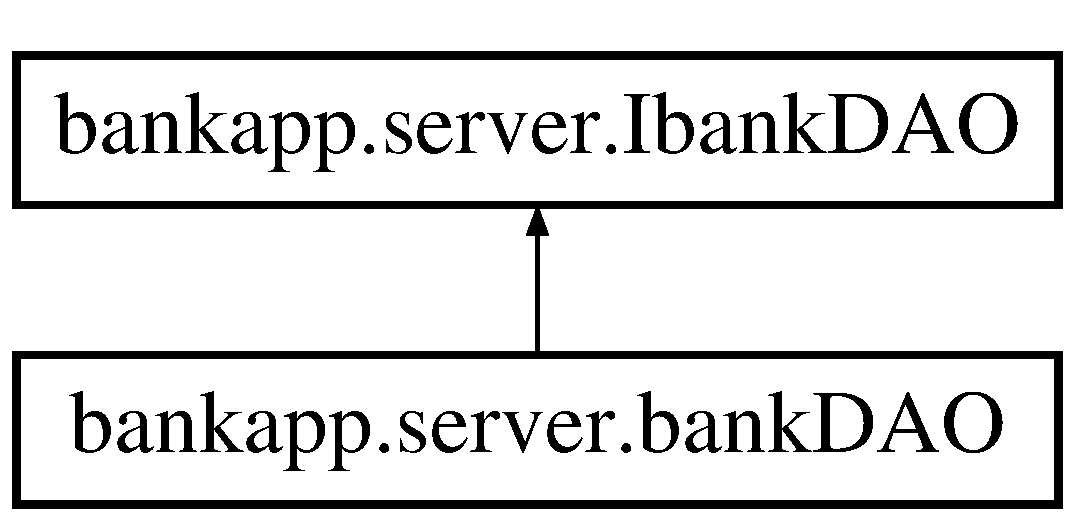
\includegraphics[height=2.000000cm]{classbankapp_1_1server_1_1bankDAO}
\end{center}
\end{figure}
\subsection*{Public Member Functions}
\begin{DoxyCompactItemize}
\item 
\mbox{\Hypertarget{classbankapp_1_1server_1_1bankDAO_a974c7da6eea192fb2f94a98a66e5068a}\label{classbankapp_1_1server_1_1bankDAO_a974c7da6eea192fb2f94a98a66e5068a}} 
\hyperlink{classbankapp_1_1server_1_1bankDAO_a974c7da6eea192fb2f94a98a66e5068a}{bank\+D\+AO} ()
\begin{DoxyCompactList}\small\item\em Constractore for class \hyperlink{classbankapp_1_1server_1_1bankDAO}{bank\+D\+AO}. \end{DoxyCompactList}\item 
\hyperlink{classbankapp_1_1server_1_1User}{User} \hyperlink{classbankapp_1_1server_1_1bankDAO_af952db62263ca6ebda3130336e63f941}{get\+User} (String username)
\begin{DoxyCompactList}\small\item\em Function to get user identified by a username giving as a param. \end{DoxyCompactList}\item 
void \hyperlink{classbankapp_1_1server_1_1bankDAO_a2026e5f30e2342995dddfc654a37d640}{store\+User} (\hyperlink{classbankapp_1_1server_1_1User}{User} user)
\begin{DoxyCompactList}\small\item\em Store a new user. \end{DoxyCompactList}\item 
void \hyperlink{classbankapp_1_1server_1_1bankDAO_ab3ed5a9b972ea31ebc023596efecb2d1}{update\+User} (\hyperlink{classbankapp_1_1server_1_1User}{User} user)
\begin{DoxyCompactList}\small\item\em update a existing user \end{DoxyCompactList}\item 
void \hyperlink{classbankapp_1_1server_1_1bankDAO_a0023f065d21c23dd9b952339fd832d7e}{store\+Account} (Account acc)
\begin{DoxyCompactList}\small\item\em Store a new amount. \end{DoxyCompactList}\item 
void \hyperlink{classbankapp_1_1server_1_1bankDAO_a22f03ae02432bc82af70d212a7a8cdba}{update\+Account} (Account acc)
\begin{DoxyCompactList}\small\item\em update an existing amount \end{DoxyCompactList}\end{DoxyCompactItemize}


\subsection{Detailed Description}
This is the bank D\+AO Class. 

\begin{DoxyAuthor}{Author}
B\+I\+C\+H\+RI 
\end{DoxyAuthor}
\begin{DoxyDate}{Date}
05-\/17-\/2017 
\end{DoxyDate}


\subsection{Member Function Documentation}
\mbox{\Hypertarget{classbankapp_1_1server_1_1bankDAO_af952db62263ca6ebda3130336e63f941}\label{classbankapp_1_1server_1_1bankDAO_af952db62263ca6ebda3130336e63f941}} 
\index{bankapp\+::server\+::bank\+D\+AO@{bankapp\+::server\+::bank\+D\+AO}!get\+User@{get\+User}}
\index{get\+User@{get\+User}!bankapp\+::server\+::bank\+D\+AO@{bankapp\+::server\+::bank\+D\+AO}}
\subsubsection{\texorpdfstring{get\+User()}{getUser()}}
{\footnotesize\ttfamily \hyperlink{classbankapp_1_1server_1_1User}{User} bankapp.\+server.\+bank\+D\+A\+O.\+get\+User (\begin{DoxyParamCaption}\item[{String}]{username }\end{DoxyParamCaption})}



Function to get user identified by a username giving as a param. 


\begin{DoxyParams}{Parameters}
{\em username} & \\
\hline
\end{DoxyParams}
\begin{DoxyReturn}{Returns}
user 
\end{DoxyReturn}


Implements \hyperlink{interfacebankapp_1_1server_1_1IbankDAO_a11bbbf14695bce77b2932f36fdb79bd8}{bankapp.\+server.\+Ibank\+D\+AO}.

\mbox{\Hypertarget{classbankapp_1_1server_1_1bankDAO_a0023f065d21c23dd9b952339fd832d7e}\label{classbankapp_1_1server_1_1bankDAO_a0023f065d21c23dd9b952339fd832d7e}} 
\index{bankapp\+::server\+::bank\+D\+AO@{bankapp\+::server\+::bank\+D\+AO}!store\+Account@{store\+Account}}
\index{store\+Account@{store\+Account}!bankapp\+::server\+::bank\+D\+AO@{bankapp\+::server\+::bank\+D\+AO}}
\subsubsection{\texorpdfstring{store\+Account()}{storeAccount()}}
{\footnotesize\ttfamily void bankapp.\+server.\+bank\+D\+A\+O.\+store\+Account (\begin{DoxyParamCaption}\item[{Account}]{acc }\end{DoxyParamCaption})}



Store a new amount. 


\begin{DoxyParams}{Parameters}
{\em acc} & \\
\hline
\end{DoxyParams}


Implements \hyperlink{interfacebankapp_1_1server_1_1IbankDAO_a6631fb11c78a48b05a743e4f7f2757ef}{bankapp.\+server.\+Ibank\+D\+AO}.

\mbox{\Hypertarget{classbankapp_1_1server_1_1bankDAO_a2026e5f30e2342995dddfc654a37d640}\label{classbankapp_1_1server_1_1bankDAO_a2026e5f30e2342995dddfc654a37d640}} 
\index{bankapp\+::server\+::bank\+D\+AO@{bankapp\+::server\+::bank\+D\+AO}!store\+User@{store\+User}}
\index{store\+User@{store\+User}!bankapp\+::server\+::bank\+D\+AO@{bankapp\+::server\+::bank\+D\+AO}}
\subsubsection{\texorpdfstring{store\+User()}{storeUser()}}
{\footnotesize\ttfamily void bankapp.\+server.\+bank\+D\+A\+O.\+store\+User (\begin{DoxyParamCaption}\item[{\hyperlink{classbankapp_1_1server_1_1User}{User}}]{user }\end{DoxyParamCaption})}



Store a new user. 


\begin{DoxyParams}{Parameters}
{\em user} & \\
\hline
\end{DoxyParams}


Implements \hyperlink{interfacebankapp_1_1server_1_1IbankDAO_a9cb41e7c04366f4ec9cfcb74d43ee37f}{bankapp.\+server.\+Ibank\+D\+AO}.

\mbox{\Hypertarget{classbankapp_1_1server_1_1bankDAO_a22f03ae02432bc82af70d212a7a8cdba}\label{classbankapp_1_1server_1_1bankDAO_a22f03ae02432bc82af70d212a7a8cdba}} 
\index{bankapp\+::server\+::bank\+D\+AO@{bankapp\+::server\+::bank\+D\+AO}!update\+Account@{update\+Account}}
\index{update\+Account@{update\+Account}!bankapp\+::server\+::bank\+D\+AO@{bankapp\+::server\+::bank\+D\+AO}}
\subsubsection{\texorpdfstring{update\+Account()}{updateAccount()}}
{\footnotesize\ttfamily void bankapp.\+server.\+bank\+D\+A\+O.\+update\+Account (\begin{DoxyParamCaption}\item[{Account}]{acc }\end{DoxyParamCaption})}



update an existing amount 


\begin{DoxyParams}{Parameters}
{\em acc} & \\
\hline
\end{DoxyParams}


Implements \hyperlink{interfacebankapp_1_1server_1_1IbankDAO_a0ee7aa6b093e2695955296dd72411b0c}{bankapp.\+server.\+Ibank\+D\+AO}.

\mbox{\Hypertarget{classbankapp_1_1server_1_1bankDAO_ab3ed5a9b972ea31ebc023596efecb2d1}\label{classbankapp_1_1server_1_1bankDAO_ab3ed5a9b972ea31ebc023596efecb2d1}} 
\index{bankapp\+::server\+::bank\+D\+AO@{bankapp\+::server\+::bank\+D\+AO}!update\+User@{update\+User}}
\index{update\+User@{update\+User}!bankapp\+::server\+::bank\+D\+AO@{bankapp\+::server\+::bank\+D\+AO}}
\subsubsection{\texorpdfstring{update\+User()}{updateUser()}}
{\footnotesize\ttfamily void bankapp.\+server.\+bank\+D\+A\+O.\+update\+User (\begin{DoxyParamCaption}\item[{\hyperlink{classbankapp_1_1server_1_1User}{User}}]{user }\end{DoxyParamCaption})}



update a existing user 


\begin{DoxyParams}{Parameters}
{\em user} & \\
\hline
\end{DoxyParams}


Implements \hyperlink{interfacebankapp_1_1server_1_1IbankDAO_a5c38ce2000e71e9c9892bf2d357103bc}{bankapp.\+server.\+Ibank\+D\+AO}.



The documentation for this class was generated from the following file\+:\begin{DoxyCompactItemize}
\item 
Bank\+App/src/main/java/bankapp/server/bank\+D\+A\+O.\+java\end{DoxyCompactItemize}

\hypertarget{classbankapp_1_1server_1_1bankServer}{}\section{bankapp.\+server.\+bank\+Server Class Reference}
\label{classbankapp_1_1server_1_1bankServer}\index{bankapp.\+server.\+bank\+Server@{bankapp.\+server.\+bank\+Server}}


This is the bank server Class.  


\subsection*{Static Public Member Functions}
\begin{DoxyCompactItemize}
\item 
static void \hyperlink{classbankapp_1_1server_1_1bankServer_aca6d24bb05576a3668a4421453785f90}{main} (String args\mbox{[}$\,$\mbox{]})
\begin{DoxyCompactList}\small\item\em main function that will do the server hundling \end{DoxyCompactList}\end{DoxyCompactItemize}


\subsection{Detailed Description}
This is the bank server Class. 

\begin{DoxyAuthor}{Author}
B\+I\+C\+H\+RI 
\end{DoxyAuthor}
\begin{DoxyDate}{Date}
05-\/17-\/2017 
\end{DoxyDate}


\subsection{Member Function Documentation}
\mbox{\Hypertarget{classbankapp_1_1server_1_1bankServer_aca6d24bb05576a3668a4421453785f90}\label{classbankapp_1_1server_1_1bankServer_aca6d24bb05576a3668a4421453785f90}} 
\index{bankapp\+::server\+::bank\+Server@{bankapp\+::server\+::bank\+Server}!main@{main}}
\index{main@{main}!bankapp\+::server\+::bank\+Server@{bankapp\+::server\+::bank\+Server}}
\subsubsection{\texorpdfstring{main()}{main()}}
{\footnotesize\ttfamily static void bankapp.\+server.\+bank\+Server.\+main (\begin{DoxyParamCaption}\item[{String}]{args\mbox{[}$\,$\mbox{]} }\end{DoxyParamCaption})\hspace{0.3cm}{\ttfamily [static]}}



main function that will do the server hundling 


\begin{DoxyParams}{Parameters}
{\em args} & \\
\hline
\end{DoxyParams}


The documentation for this class was generated from the following file\+:\begin{DoxyCompactItemize}
\item 
Bank\+App/src/main/java/bankapp/server/bank\+Server.\+java\end{DoxyCompactItemize}

\hypertarget{classbankapp_1_1server_1_1BManager}{}\section{bankapp.\+server.\+B\+Manager Class Reference}
\label{classbankapp_1_1server_1_1BManager}\index{bankapp.\+server.\+B\+Manager@{bankapp.\+server.\+B\+Manager}}


This is the bank manger Class extends Unicast\+Remote\+Object and implements \hyperlink{interfacebankapp_1_1server_1_1IBManager}{I\+B\+Manager}.  


Inheritance diagram for bankapp.\+server.\+B\+Manager\+:\begin{figure}[H]
\begin{center}
\leavevmode
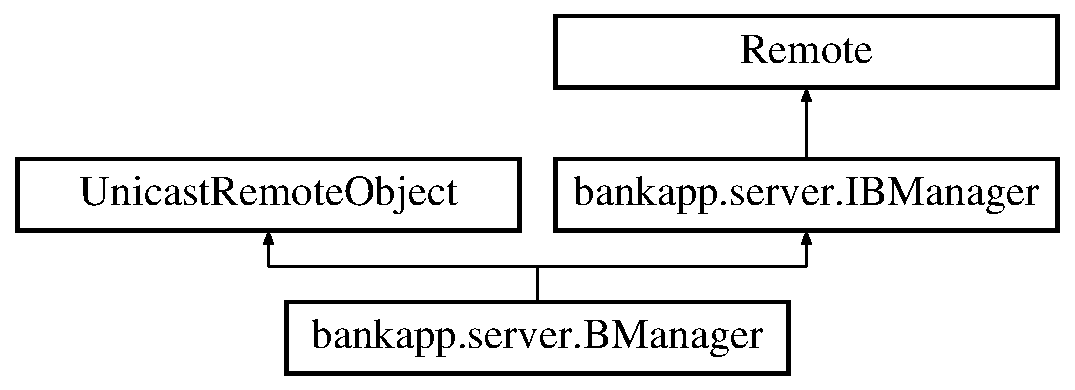
\includegraphics[height=3.000000cm]{classbankapp_1_1server_1_1BManager}
\end{center}
\end{figure}
\subsection*{Public Member Functions}
\begin{DoxyCompactItemize}
\item 
\hyperlink{classbankapp_1_1server_1_1BManager_aa7f45d3eddae4e91afaf2b19275b0c7e}{B\+Manager} (String server\+Address, String port0, String serv\+Name)  throws Remote\+Exception 
\begin{DoxyCompactList}\small\item\em \hyperlink{classbankapp_1_1server_1_1BManager}{B\+Manager} Constructor and also store an new user. \end{DoxyCompactList}\item 
boolean \hyperlink{classbankapp_1_1server_1_1BManager_abdeb5e23b534babeed067c3667fcafd3}{login} (String username, String pass)  throws Remote\+Exception 
\begin{DoxyCompactList}\small\item\em Function Login as a bank manager allow or deny access. \end{DoxyCompactList}\end{DoxyCompactItemize}


\subsection{Detailed Description}
This is the bank manger Class extends Unicast\+Remote\+Object and implements \hyperlink{interfacebankapp_1_1server_1_1IBManager}{I\+B\+Manager}. 

\begin{DoxyAuthor}{Author}
B\+I\+C\+H\+RI 
\end{DoxyAuthor}
\begin{DoxyDate}{Date}
05-\/17-\/2017 
\end{DoxyDate}


\subsection{Constructor \& Destructor Documentation}
\mbox{\Hypertarget{classbankapp_1_1server_1_1BManager_aa7f45d3eddae4e91afaf2b19275b0c7e}\label{classbankapp_1_1server_1_1BManager_aa7f45d3eddae4e91afaf2b19275b0c7e}} 
\index{bankapp\+::server\+::\+B\+Manager@{bankapp\+::server\+::\+B\+Manager}!B\+Manager@{B\+Manager}}
\index{B\+Manager@{B\+Manager}!bankapp\+::server\+::\+B\+Manager@{bankapp\+::server\+::\+B\+Manager}}
\subsubsection{\texorpdfstring{B\+Manager()}{BManager()}}
{\footnotesize\ttfamily bankapp.\+server.\+B\+Manager.\+B\+Manager (\begin{DoxyParamCaption}\item[{String}]{server\+Address,  }\item[{String}]{port0,  }\item[{String}]{serv\+Name }\end{DoxyParamCaption}) throws Remote\+Exception}



\hyperlink{classbankapp_1_1server_1_1BManager}{B\+Manager} Constructor and also store an new user. 


\begin{DoxyParams}{Parameters}
{\em server\+Address} & \\
\hline
{\em port0} & \\
\hline
{\em serv\+Name} & \\
\hline
\end{DoxyParams}

\begin{DoxyExceptions}{Exceptions}
{\em Remote\+Exception} & \\
\hline
\end{DoxyExceptions}


\subsection{Member Function Documentation}
\mbox{\Hypertarget{classbankapp_1_1server_1_1BManager_abdeb5e23b534babeed067c3667fcafd3}\label{classbankapp_1_1server_1_1BManager_abdeb5e23b534babeed067c3667fcafd3}} 
\index{bankapp\+::server\+::\+B\+Manager@{bankapp\+::server\+::\+B\+Manager}!login@{login}}
\index{login@{login}!bankapp\+::server\+::\+B\+Manager@{bankapp\+::server\+::\+B\+Manager}}
\subsubsection{\texorpdfstring{login()}{login()}}
{\footnotesize\ttfamily boolean bankapp.\+server.\+B\+Manager.\+login (\begin{DoxyParamCaption}\item[{String}]{username,  }\item[{String}]{pass }\end{DoxyParamCaption}) throws Remote\+Exception}



Function Login as a bank manager allow or deny access. 


\begin{DoxyParams}{Parameters}
{\em username} & \\
\hline
{\em pass} & \\
\hline
\end{DoxyParams}
\begin{DoxyReturn}{Returns}
false 
\end{DoxyReturn}

\begin{DoxyExceptions}{Exceptions}
{\em Remote\+Exception} & \\
\hline
\end{DoxyExceptions}


Implements \hyperlink{interfacebankapp_1_1server_1_1IBManager_a29f3426c104732dda17dc8b215b746e1}{bankapp.\+server.\+I\+B\+Manager}.



The documentation for this class was generated from the following file\+:\begin{DoxyCompactItemize}
\item 
Bank\+App/src/main/java/bankapp/server/B\+Manager.\+java\end{DoxyCompactItemize}

\hypertarget{interfacebankapp_1_1server_1_1IbankDAO}{}\section{bankapp.\+server.\+Ibank\+D\+AO Interface Reference}
\label{interfacebankapp_1_1server_1_1IbankDAO}\index{bankapp.\+server.\+Ibank\+D\+AO@{bankapp.\+server.\+Ibank\+D\+AO}}


Interface \hyperlink{interfacebankapp_1_1server_1_1IbankDAO}{Ibank\+D\+AO} to set function names and params.  


Inheritance diagram for bankapp.\+server.\+Ibank\+D\+AO\+:\begin{figure}[H]
\begin{center}
\leavevmode
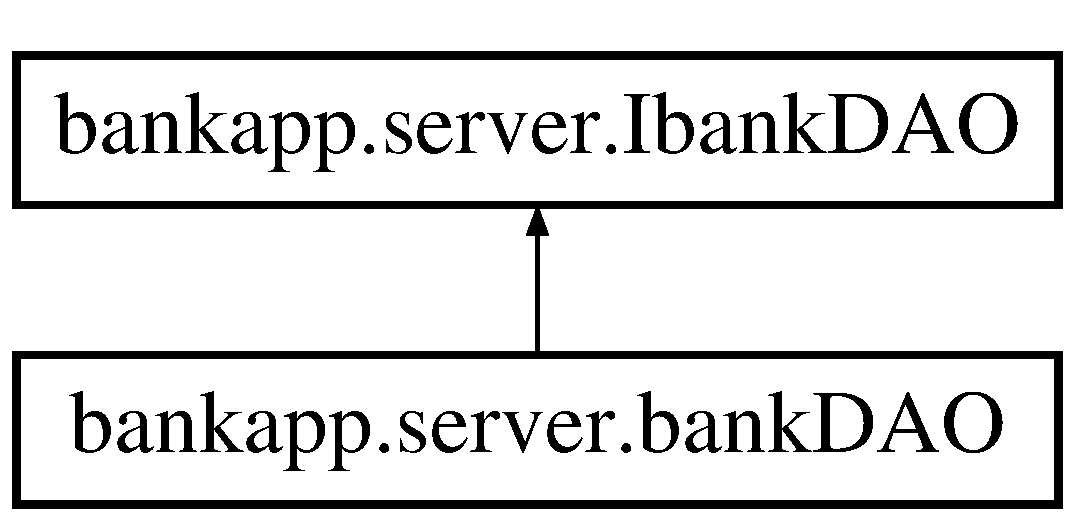
\includegraphics[height=2.000000cm]{interfacebankapp_1_1server_1_1IbankDAO}
\end{center}
\end{figure}
\subsection*{Public Member Functions}
\begin{DoxyCompactItemize}
\item 
\hyperlink{classbankapp_1_1server_1_1User}{User} \hyperlink{interfacebankapp_1_1server_1_1IbankDAO_a11bbbf14695bce77b2932f36fdb79bd8}{get\+User} (String username)
\begin{DoxyCompactList}\small\item\em function name and params \end{DoxyCompactList}\item 
void \hyperlink{interfacebankapp_1_1server_1_1IbankDAO_a9cb41e7c04366f4ec9cfcb74d43ee37f}{store\+User} (\hyperlink{classbankapp_1_1server_1_1User}{User} user)
\begin{DoxyCompactList}\small\item\em function name and params \end{DoxyCompactList}\item 
void \hyperlink{interfacebankapp_1_1server_1_1IbankDAO_a5c38ce2000e71e9c9892bf2d357103bc}{update\+User} (\hyperlink{classbankapp_1_1server_1_1User}{User} user)
\begin{DoxyCompactList}\small\item\em function name and params \end{DoxyCompactList}\item 
void \hyperlink{interfacebankapp_1_1server_1_1IbankDAO_a6631fb11c78a48b05a743e4f7f2757ef}{store\+Account} (Account acc)
\begin{DoxyCompactList}\small\item\em function name and params \end{DoxyCompactList}\item 
void \hyperlink{interfacebankapp_1_1server_1_1IbankDAO_a0ee7aa6b093e2695955296dd72411b0c}{update\+Account} (Account acc)
\begin{DoxyCompactList}\small\item\em function name and params \end{DoxyCompactList}\end{DoxyCompactItemize}


\subsection{Detailed Description}
Interface \hyperlink{interfacebankapp_1_1server_1_1IbankDAO}{Ibank\+D\+AO} to set function names and params. 

\begin{DoxyAuthor}{Author}
B\+I\+C\+H\+RI 
\end{DoxyAuthor}
\begin{DoxyDate}{Date}
05-\/17-\/2017 
\end{DoxyDate}


\subsection{Member Function Documentation}
\mbox{\Hypertarget{interfacebankapp_1_1server_1_1IbankDAO_a11bbbf14695bce77b2932f36fdb79bd8}\label{interfacebankapp_1_1server_1_1IbankDAO_a11bbbf14695bce77b2932f36fdb79bd8}} 
\index{bankapp\+::server\+::\+Ibank\+D\+AO@{bankapp\+::server\+::\+Ibank\+D\+AO}!get\+User@{get\+User}}
\index{get\+User@{get\+User}!bankapp\+::server\+::\+Ibank\+D\+AO@{bankapp\+::server\+::\+Ibank\+D\+AO}}
\subsubsection{\texorpdfstring{get\+User()}{getUser()}}
{\footnotesize\ttfamily \hyperlink{classbankapp_1_1server_1_1User}{User} bankapp.\+server.\+Ibank\+D\+A\+O.\+get\+User (\begin{DoxyParamCaption}\item[{String}]{username }\end{DoxyParamCaption})}



function name and params 


\begin{DoxyParams}{Parameters}
{\em username} & \\
\hline
\end{DoxyParams}
\begin{DoxyReturn}{Returns}
user 
\end{DoxyReturn}


Implemented in \hyperlink{classbankapp_1_1server_1_1bankDAO_af952db62263ca6ebda3130336e63f941}{bankapp.\+server.\+bank\+D\+AO}.

\mbox{\Hypertarget{interfacebankapp_1_1server_1_1IbankDAO_a6631fb11c78a48b05a743e4f7f2757ef}\label{interfacebankapp_1_1server_1_1IbankDAO_a6631fb11c78a48b05a743e4f7f2757ef}} 
\index{bankapp\+::server\+::\+Ibank\+D\+AO@{bankapp\+::server\+::\+Ibank\+D\+AO}!store\+Account@{store\+Account}}
\index{store\+Account@{store\+Account}!bankapp\+::server\+::\+Ibank\+D\+AO@{bankapp\+::server\+::\+Ibank\+D\+AO}}
\subsubsection{\texorpdfstring{store\+Account()}{storeAccount()}}
{\footnotesize\ttfamily void bankapp.\+server.\+Ibank\+D\+A\+O.\+store\+Account (\begin{DoxyParamCaption}\item[{Account}]{acc }\end{DoxyParamCaption})}



function name and params 


\begin{DoxyParams}{Parameters}
{\em acc} & \\
\hline
\end{DoxyParams}


Implemented in \hyperlink{classbankapp_1_1server_1_1bankDAO_a0023f065d21c23dd9b952339fd832d7e}{bankapp.\+server.\+bank\+D\+AO}.

\mbox{\Hypertarget{interfacebankapp_1_1server_1_1IbankDAO_a9cb41e7c04366f4ec9cfcb74d43ee37f}\label{interfacebankapp_1_1server_1_1IbankDAO_a9cb41e7c04366f4ec9cfcb74d43ee37f}} 
\index{bankapp\+::server\+::\+Ibank\+D\+AO@{bankapp\+::server\+::\+Ibank\+D\+AO}!store\+User@{store\+User}}
\index{store\+User@{store\+User}!bankapp\+::server\+::\+Ibank\+D\+AO@{bankapp\+::server\+::\+Ibank\+D\+AO}}
\subsubsection{\texorpdfstring{store\+User()}{storeUser()}}
{\footnotesize\ttfamily void bankapp.\+server.\+Ibank\+D\+A\+O.\+store\+User (\begin{DoxyParamCaption}\item[{\hyperlink{classbankapp_1_1server_1_1User}{User}}]{user }\end{DoxyParamCaption})}



function name and params 


\begin{DoxyParams}{Parameters}
{\em user} & \\
\hline
\end{DoxyParams}


Implemented in \hyperlink{classbankapp_1_1server_1_1bankDAO_a2026e5f30e2342995dddfc654a37d640}{bankapp.\+server.\+bank\+D\+AO}.

\mbox{\Hypertarget{interfacebankapp_1_1server_1_1IbankDAO_a0ee7aa6b093e2695955296dd72411b0c}\label{interfacebankapp_1_1server_1_1IbankDAO_a0ee7aa6b093e2695955296dd72411b0c}} 
\index{bankapp\+::server\+::\+Ibank\+D\+AO@{bankapp\+::server\+::\+Ibank\+D\+AO}!update\+Account@{update\+Account}}
\index{update\+Account@{update\+Account}!bankapp\+::server\+::\+Ibank\+D\+AO@{bankapp\+::server\+::\+Ibank\+D\+AO}}
\subsubsection{\texorpdfstring{update\+Account()}{updateAccount()}}
{\footnotesize\ttfamily void bankapp.\+server.\+Ibank\+D\+A\+O.\+update\+Account (\begin{DoxyParamCaption}\item[{Account}]{acc }\end{DoxyParamCaption})}



function name and params 


\begin{DoxyParams}{Parameters}
{\em acc} & \\
\hline
\end{DoxyParams}


Implemented in \hyperlink{classbankapp_1_1server_1_1bankDAO_a22f03ae02432bc82af70d212a7a8cdba}{bankapp.\+server.\+bank\+D\+AO}.

\mbox{\Hypertarget{interfacebankapp_1_1server_1_1IbankDAO_a5c38ce2000e71e9c9892bf2d357103bc}\label{interfacebankapp_1_1server_1_1IbankDAO_a5c38ce2000e71e9c9892bf2d357103bc}} 
\index{bankapp\+::server\+::\+Ibank\+D\+AO@{bankapp\+::server\+::\+Ibank\+D\+AO}!update\+User@{update\+User}}
\index{update\+User@{update\+User}!bankapp\+::server\+::\+Ibank\+D\+AO@{bankapp\+::server\+::\+Ibank\+D\+AO}}
\subsubsection{\texorpdfstring{update\+User()}{updateUser()}}
{\footnotesize\ttfamily void bankapp.\+server.\+Ibank\+D\+A\+O.\+update\+User (\begin{DoxyParamCaption}\item[{\hyperlink{classbankapp_1_1server_1_1User}{User}}]{user }\end{DoxyParamCaption})}



function name and params 


\begin{DoxyParams}{Parameters}
{\em user} & \\
\hline
\end{DoxyParams}


Implemented in \hyperlink{classbankapp_1_1server_1_1bankDAO_ab3ed5a9b972ea31ebc023596efecb2d1}{bankapp.\+server.\+bank\+D\+AO}.



The documentation for this interface was generated from the following file\+:\begin{DoxyCompactItemize}
\item 
Bank\+App/src/main/java/bankapp/server/Ibank\+D\+A\+O.\+java\end{DoxyCompactItemize}

\hypertarget{interfacebankapp_1_1server_1_1IBManager}{}\section{bankapp.\+server.\+I\+B\+Manager Interface Reference}
\label{interfacebankapp_1_1server_1_1IBManager}\index{bankapp.\+server.\+I\+B\+Manager@{bankapp.\+server.\+I\+B\+Manager}}


Interface \hyperlink{interfacebankapp_1_1server_1_1IBManager}{I\+B\+Manager} extends Remote to set function names and params.  


Inheritance diagram for bankapp.\+server.\+I\+B\+Manager\+:\begin{figure}[H]
\begin{center}
\leavevmode
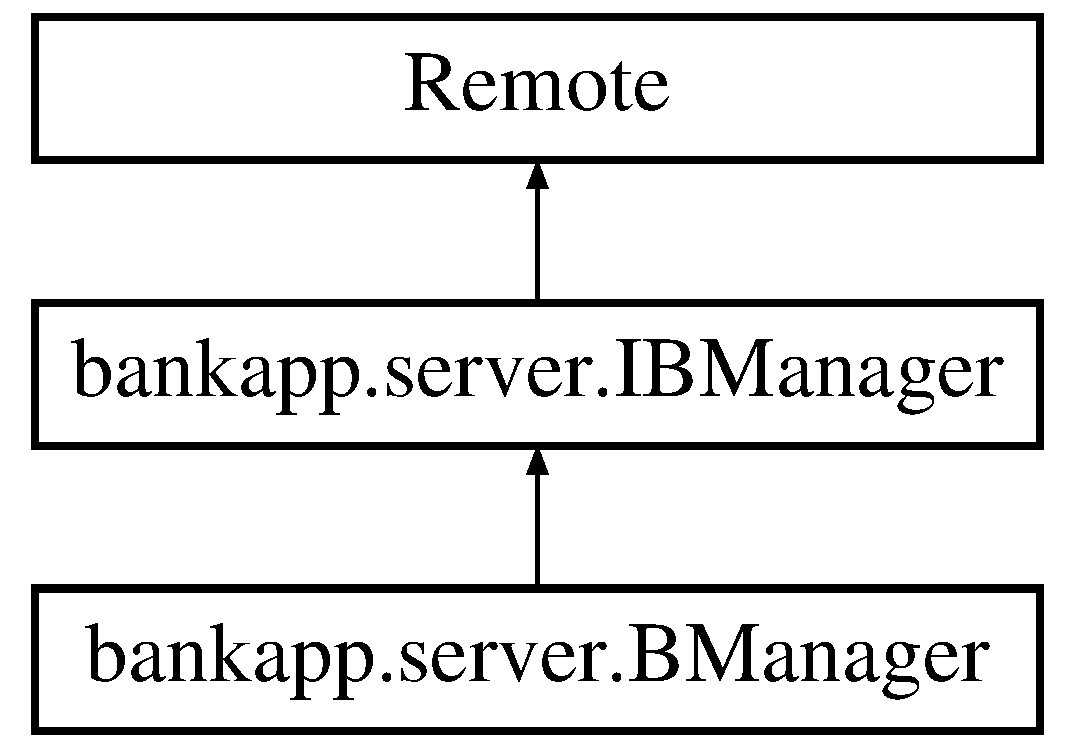
\includegraphics[height=3.000000cm]{interfacebankapp_1_1server_1_1IBManager}
\end{center}
\end{figure}
\subsection*{Public Member Functions}
\begin{DoxyCompactItemize}
\item 
boolean \hyperlink{interfacebankapp_1_1server_1_1IBManager_a29f3426c104732dda17dc8b215b746e1}{login} (String user, String pass)  throws Remote\+Exception
\begin{DoxyCompactList}\small\item\em function name and params \end{DoxyCompactList}\end{DoxyCompactItemize}


\subsection{Detailed Description}
Interface \hyperlink{interfacebankapp_1_1server_1_1IBManager}{I\+B\+Manager} extends Remote to set function names and params. 

\begin{DoxyAuthor}{Author}
B\+I\+C\+H\+RI 
\end{DoxyAuthor}
\begin{DoxyDate}{Date}
05-\/17-\/2017 
\end{DoxyDate}


\subsection{Member Function Documentation}
\mbox{\Hypertarget{interfacebankapp_1_1server_1_1IBManager_a29f3426c104732dda17dc8b215b746e1}\label{interfacebankapp_1_1server_1_1IBManager_a29f3426c104732dda17dc8b215b746e1}} 
\index{bankapp\+::server\+::\+I\+B\+Manager@{bankapp\+::server\+::\+I\+B\+Manager}!login@{login}}
\index{login@{login}!bankapp\+::server\+::\+I\+B\+Manager@{bankapp\+::server\+::\+I\+B\+Manager}}
\subsubsection{\texorpdfstring{login()}{login()}}
{\footnotesize\ttfamily boolean bankapp.\+server.\+I\+B\+Manager.\+login (\begin{DoxyParamCaption}\item[{String}]{user,  }\item[{String}]{pass }\end{DoxyParamCaption}) throws Remote\+Exception}



function name and params 


\begin{DoxyParams}{Parameters}
{\em user} & \\
\hline
{\em pass} & \\
\hline
\end{DoxyParams}
\begin{DoxyReturn}{Returns}

\end{DoxyReturn}

\begin{DoxyExceptions}{Exceptions}
{\em Remote\+Exception} & \\
\hline
\end{DoxyExceptions}


Implemented in \hyperlink{classbankapp_1_1server_1_1BManager_abdeb5e23b534babeed067c3667fcafd3}{bankapp.\+server.\+B\+Manager}.



The documentation for this interface was generated from the following file\+:\begin{DoxyCompactItemize}
\item 
Bank\+App/src/main/java/bankapp/server/I\+B\+Manager.\+java\end{DoxyCompactItemize}

\hypertarget{classbankapp_1_1client_1_1RMIServiceLocator}{}\section{bankapp.\+client.\+R\+M\+I\+Service\+Locator Class Reference}
\label{classbankapp_1_1client_1_1RMIServiceLocator}\index{bankapp.\+client.\+R\+M\+I\+Service\+Locator@{bankapp.\+client.\+R\+M\+I\+Service\+Locator}}


This is the bank R\+M\+I\+Services hundler Class.  


\subsection*{Public Member Functions}
\begin{DoxyCompactItemize}
\item 
void \hyperlink{classbankapp_1_1client_1_1RMIServiceLocator_a9a1605fa6be3933008e90db56b804007}{set\+Service} (String ip, String port, String service\+Name)
\begin{DoxyCompactList}\small\item\em set the service of an R\+MI \end{DoxyCompactList}\item 
boolean \hyperlink{classbankapp_1_1client_1_1RMIServiceLocator_a2287058ad6e7eaa5b38303c02102d740}{login} (String user, String pass)
\begin{DoxyCompactList}\small\item\em Login to R\+M\+I\+Service. \end{DoxyCompactList}\end{DoxyCompactItemize}


\subsection{Detailed Description}
This is the bank R\+M\+I\+Services hundler Class. 

\begin{DoxyAuthor}{Author}
B\+I\+C\+H\+RI 
\end{DoxyAuthor}
\begin{DoxyDate}{Date}
05-\/17-\/2017 
\end{DoxyDate}


\subsection{Member Function Documentation}
\mbox{\Hypertarget{classbankapp_1_1client_1_1RMIServiceLocator_a2287058ad6e7eaa5b38303c02102d740}\label{classbankapp_1_1client_1_1RMIServiceLocator_a2287058ad6e7eaa5b38303c02102d740}} 
\index{bankapp\+::client\+::\+R\+M\+I\+Service\+Locator@{bankapp\+::client\+::\+R\+M\+I\+Service\+Locator}!login@{login}}
\index{login@{login}!bankapp\+::client\+::\+R\+M\+I\+Service\+Locator@{bankapp\+::client\+::\+R\+M\+I\+Service\+Locator}}
\subsubsection{\texorpdfstring{login()}{login()}}
{\footnotesize\ttfamily boolean bankapp.\+client.\+R\+M\+I\+Service\+Locator.\+login (\begin{DoxyParamCaption}\item[{String}]{user,  }\item[{String}]{pass }\end{DoxyParamCaption})}



Login to R\+M\+I\+Service. 


\begin{DoxyParams}{Parameters}
{\em user} & \\
\hline
{\em pass} & \\
\hline
\end{DoxyParams}
\begin{DoxyReturn}{Returns}
false 
\end{DoxyReturn}
\mbox{\Hypertarget{classbankapp_1_1client_1_1RMIServiceLocator_a9a1605fa6be3933008e90db56b804007}\label{classbankapp_1_1client_1_1RMIServiceLocator_a9a1605fa6be3933008e90db56b804007}} 
\index{bankapp\+::client\+::\+R\+M\+I\+Service\+Locator@{bankapp\+::client\+::\+R\+M\+I\+Service\+Locator}!set\+Service@{set\+Service}}
\index{set\+Service@{set\+Service}!bankapp\+::client\+::\+R\+M\+I\+Service\+Locator@{bankapp\+::client\+::\+R\+M\+I\+Service\+Locator}}
\subsubsection{\texorpdfstring{set\+Service()}{setService()}}
{\footnotesize\ttfamily void bankapp.\+client.\+R\+M\+I\+Service\+Locator.\+set\+Service (\begin{DoxyParamCaption}\item[{String}]{ip,  }\item[{String}]{port,  }\item[{String}]{service\+Name }\end{DoxyParamCaption})}



set the service of an R\+MI 


\begin{DoxyParams}{Parameters}
{\em ip} & \\
\hline
{\em port} & \\
\hline
{\em service\+Name} & \\
\hline
\end{DoxyParams}


The documentation for this class was generated from the following file\+:\begin{DoxyCompactItemize}
\item 
Bank\+App/src/main/java/bankapp/client/R\+M\+I\+Service\+Locator.\+java\end{DoxyCompactItemize}

\hypertarget{classbankapp_1_1server_1_1User}{}\section{bankapp.\+server.\+User Class Reference}
\label{classbankapp_1_1server_1_1User}\index{bankapp.\+server.\+User@{bankapp.\+server.\+User}}


class \hyperlink{classbankapp_1_1server_1_1User}{User} contain the attributes that a user must have  


\subsection*{Public Member Functions}
\begin{DoxyCompactItemize}
\item 
\hyperlink{classbankapp_1_1server_1_1User_ae5d0c0c37ed136f1c3e7534a4af49105}{User} (String username, String pass, String email)
\begin{DoxyCompactList}\small\item\em Constractor for class \hyperlink{classbankapp_1_1server_1_1User}{User}. \end{DoxyCompactList}\item 
String \hyperlink{classbankapp_1_1server_1_1User_a891bc2d8c2b280f081178b65b029863c}{get\+Username} ()
\begin{DoxyCompactList}\small\item\em function to get the user name \end{DoxyCompactList}\item 
void \hyperlink{classbankapp_1_1server_1_1User_a928dc59410a7254dc30e433c39cf31bd}{set\+Username} (String username)
\begin{DoxyCompactList}\small\item\em functionto set the user name \end{DoxyCompactList}\item 
String \hyperlink{classbankapp_1_1server_1_1User_ac0743fe168b925a6c422586a94741cb9}{get\+Pass} ()
\begin{DoxyCompactList}\small\item\em function to get the user password \end{DoxyCompactList}\item 
void \hyperlink{classbankapp_1_1server_1_1User_a3456b274c14301835b2727b0355fbdb2}{set\+Pass} (String pass)
\begin{DoxyCompactList}\small\item\em function to set the user password \end{DoxyCompactList}\item 
String \hyperlink{classbankapp_1_1server_1_1User_a597376bdfa749415e75185e764b3e04f}{get\+Email} ()
\begin{DoxyCompactList}\small\item\em function to get the user email \end{DoxyCompactList}\item 
void \hyperlink{classbankapp_1_1server_1_1User_aef6765beb0d9556f38070c919ca7e732}{set\+Email} (String email)
\begin{DoxyCompactList}\small\item\em function to set the user email \end{DoxyCompactList}\item 
String \hyperlink{classbankapp_1_1server_1_1User_a9c6aa2df5a2c7d9cd8b4c4a228f7cbeb}{to\+String} ()
\begin{DoxyCompactList}\small\item\em function to get the user name \end{DoxyCompactList}\end{DoxyCompactItemize}


\subsection{Detailed Description}
class \hyperlink{classbankapp_1_1server_1_1User}{User} contain the attributes that a user must have 

\begin{DoxyAuthor}{Author}
B\+I\+C\+H\+RI 
\end{DoxyAuthor}
\begin{DoxyDate}{Date}
05-\/17-\/2017 
\end{DoxyDate}


\subsection{Constructor \& Destructor Documentation}
\mbox{\Hypertarget{classbankapp_1_1server_1_1User_ae5d0c0c37ed136f1c3e7534a4af49105}\label{classbankapp_1_1server_1_1User_ae5d0c0c37ed136f1c3e7534a4af49105}} 
\index{bankapp\+::server\+::\+User@{bankapp\+::server\+::\+User}!User@{User}}
\index{User@{User}!bankapp\+::server\+::\+User@{bankapp\+::server\+::\+User}}
\subsubsection{\texorpdfstring{User()}{User()}}
{\footnotesize\ttfamily bankapp.\+server.\+User.\+User (\begin{DoxyParamCaption}\item[{String}]{username,  }\item[{String}]{pass,  }\item[{String}]{email }\end{DoxyParamCaption})}



Constractor for class \hyperlink{classbankapp_1_1server_1_1User}{User}. 


\begin{DoxyParams}{Parameters}
{\em username} & \\
\hline
{\em pass} & \\
\hline
{\em email} & \\
\hline
\end{DoxyParams}


\subsection{Member Function Documentation}
\mbox{\Hypertarget{classbankapp_1_1server_1_1User_a597376bdfa749415e75185e764b3e04f}\label{classbankapp_1_1server_1_1User_a597376bdfa749415e75185e764b3e04f}} 
\index{bankapp\+::server\+::\+User@{bankapp\+::server\+::\+User}!get\+Email@{get\+Email}}
\index{get\+Email@{get\+Email}!bankapp\+::server\+::\+User@{bankapp\+::server\+::\+User}}
\subsubsection{\texorpdfstring{get\+Email()}{getEmail()}}
{\footnotesize\ttfamily String bankapp.\+server.\+User.\+get\+Email (\begin{DoxyParamCaption}{ }\end{DoxyParamCaption})}



function to get the user email 

\begin{DoxyReturn}{Returns}
email 
\end{DoxyReturn}
\mbox{\Hypertarget{classbankapp_1_1server_1_1User_ac0743fe168b925a6c422586a94741cb9}\label{classbankapp_1_1server_1_1User_ac0743fe168b925a6c422586a94741cb9}} 
\index{bankapp\+::server\+::\+User@{bankapp\+::server\+::\+User}!get\+Pass@{get\+Pass}}
\index{get\+Pass@{get\+Pass}!bankapp\+::server\+::\+User@{bankapp\+::server\+::\+User}}
\subsubsection{\texorpdfstring{get\+Pass()}{getPass()}}
{\footnotesize\ttfamily String bankapp.\+server.\+User.\+get\+Pass (\begin{DoxyParamCaption}{ }\end{DoxyParamCaption})}



function to get the user password 

\begin{DoxyReturn}{Returns}
pass 
\end{DoxyReturn}
\mbox{\Hypertarget{classbankapp_1_1server_1_1User_a891bc2d8c2b280f081178b65b029863c}\label{classbankapp_1_1server_1_1User_a891bc2d8c2b280f081178b65b029863c}} 
\index{bankapp\+::server\+::\+User@{bankapp\+::server\+::\+User}!get\+Username@{get\+Username}}
\index{get\+Username@{get\+Username}!bankapp\+::server\+::\+User@{bankapp\+::server\+::\+User}}
\subsubsection{\texorpdfstring{get\+Username()}{getUsername()}}
{\footnotesize\ttfamily String bankapp.\+server.\+User.\+get\+Username (\begin{DoxyParamCaption}{ }\end{DoxyParamCaption})}



function to get the user name 

\begin{DoxyReturn}{Returns}
username 
\end{DoxyReturn}
\mbox{\Hypertarget{classbankapp_1_1server_1_1User_aef6765beb0d9556f38070c919ca7e732}\label{classbankapp_1_1server_1_1User_aef6765beb0d9556f38070c919ca7e732}} 
\index{bankapp\+::server\+::\+User@{bankapp\+::server\+::\+User}!set\+Email@{set\+Email}}
\index{set\+Email@{set\+Email}!bankapp\+::server\+::\+User@{bankapp\+::server\+::\+User}}
\subsubsection{\texorpdfstring{set\+Email()}{setEmail()}}
{\footnotesize\ttfamily void bankapp.\+server.\+User.\+set\+Email (\begin{DoxyParamCaption}\item[{String}]{email }\end{DoxyParamCaption})}



function to set the user email 


\begin{DoxyParams}{Parameters}
{\em email} & \\
\hline
\end{DoxyParams}
\mbox{\Hypertarget{classbankapp_1_1server_1_1User_a3456b274c14301835b2727b0355fbdb2}\label{classbankapp_1_1server_1_1User_a3456b274c14301835b2727b0355fbdb2}} 
\index{bankapp\+::server\+::\+User@{bankapp\+::server\+::\+User}!set\+Pass@{set\+Pass}}
\index{set\+Pass@{set\+Pass}!bankapp\+::server\+::\+User@{bankapp\+::server\+::\+User}}
\subsubsection{\texorpdfstring{set\+Pass()}{setPass()}}
{\footnotesize\ttfamily void bankapp.\+server.\+User.\+set\+Pass (\begin{DoxyParamCaption}\item[{String}]{pass }\end{DoxyParamCaption})}



function to set the user password 


\begin{DoxyParams}{Parameters}
{\em pass} & \\
\hline
\end{DoxyParams}
\mbox{\Hypertarget{classbankapp_1_1server_1_1User_a928dc59410a7254dc30e433c39cf31bd}\label{classbankapp_1_1server_1_1User_a928dc59410a7254dc30e433c39cf31bd}} 
\index{bankapp\+::server\+::\+User@{bankapp\+::server\+::\+User}!set\+Username@{set\+Username}}
\index{set\+Username@{set\+Username}!bankapp\+::server\+::\+User@{bankapp\+::server\+::\+User}}
\subsubsection{\texorpdfstring{set\+Username()}{setUsername()}}
{\footnotesize\ttfamily void bankapp.\+server.\+User.\+set\+Username (\begin{DoxyParamCaption}\item[{String}]{username }\end{DoxyParamCaption})}



functionto set the user name 


\begin{DoxyParams}{Parameters}
{\em username} & \\
\hline
\end{DoxyParams}
\mbox{\Hypertarget{classbankapp_1_1server_1_1User_a9c6aa2df5a2c7d9cd8b4c4a228f7cbeb}\label{classbankapp_1_1server_1_1User_a9c6aa2df5a2c7d9cd8b4c4a228f7cbeb}} 
\index{bankapp\+::server\+::\+User@{bankapp\+::server\+::\+User}!to\+String@{to\+String}}
\index{to\+String@{to\+String}!bankapp\+::server\+::\+User@{bankapp\+::server\+::\+User}}
\subsubsection{\texorpdfstring{to\+String()}{toString()}}
{\footnotesize\ttfamily String bankapp.\+server.\+User.\+to\+String (\begin{DoxyParamCaption}{ }\end{DoxyParamCaption})}



function to get the user name 

\begin{DoxyReturn}{Returns}
username 
\end{DoxyReturn}


The documentation for this class was generated from the following file\+:\begin{DoxyCompactItemize}
\item 
Bank\+App/src/main/java/bankapp/server/User.\+java\end{DoxyCompactItemize}

%--- End generated contents ---

% Index
\backmatter
\newpage
\phantomsection
\clearemptydoublepage
\addcontentsline{toc}{chapter}{Index}
\printindex

\end{document}
